\documentclass[]{article}
\usepackage{lmodern}
\usepackage{amssymb,amsmath}
\usepackage{ifxetex,ifluatex}
\usepackage{fixltx2e} % provides \textsubscript
\ifnum 0\ifxetex 1\fi\ifluatex 1\fi=0 % if pdftex
  \usepackage[T1]{fontenc}
  \usepackage[utf8]{inputenc}
\else % if luatex or xelatex
  \ifxetex
    \usepackage{mathspec}
  \else
    \usepackage{fontspec}
  \fi
  \defaultfontfeatures{Ligatures=TeX,Scale=MatchLowercase}
\fi
% use upquote if available, for straight quotes in verbatim environments
\IfFileExists{upquote.sty}{\usepackage{upquote}}{}
% use microtype if available
\IfFileExists{microtype.sty}{%
\usepackage{microtype}
\UseMicrotypeSet[protrusion]{basicmath} % disable protrusion for tt fonts
}{}
\usepackage[unicode=true]{hyperref}
\hypersetup{
            pdfborder={0 0 0},
            breaklinks=true}
\urlstyle{same}  % don't use monospace font for urls
\usepackage{graphicx,grffile}
\makeatletter
\def\maxwidth{\ifdim\Gin@nat@width>\linewidth\linewidth\else\Gin@nat@width\fi}
\def\maxheight{\ifdim\Gin@nat@height>\textheight\textheight\else\Gin@nat@height\fi}
\makeatother
% Scale images if necessary, so that they will not overflow the page
% margins by default, and it is still possible to overwrite the defaults
% using explicit options in \includegraphics[width, height, ...]{}
\setkeys{Gin}{width=\maxwidth,height=\maxheight,keepaspectratio}
\IfFileExists{parskip.sty}{%
\usepackage{parskip}
}{% else
\setlength{\parindent}{0pt}
\setlength{\parskip}{6pt plus 2pt minus 1pt}
}
\setlength{\emergencystretch}{3em}  % prevent overfull lines
\providecommand{\tightlist}{%
  \setlength{\itemsep}{0pt}\setlength{\parskip}{0pt}}
\setcounter{secnumdepth}{0}
% Redefines (sub)paragraphs to behave more like sections
\ifx\paragraph\undefined\else
\let\oldparagraph\paragraph
\renewcommand{\paragraph}[1]{\oldparagraph{#1}\mbox{}}
\fi
\ifx\subparagraph\undefined\else
\let\oldsubparagraph\subparagraph
\renewcommand{\subparagraph}[1]{\oldsubparagraph{#1}\mbox{}}
\fi

\date{}

\begin{document}

\section{SmartCalc v1.0}\label{smartcalc-v1.0}

\subsection{Contents}\label{contents}

\begin{enumerate}
\def\labelenumi{\arabic{enumi}.}
\setcounter{enumi}{-1}
\tightlist
\item
  \protect\hyperlink{installation}{Installation}
\item
  \protect\hyperlink{calc}{Calculator}
\item
  \protect\hyperlink{deposit}{Deposit calculator}
\item
  \protect\hyperlink{credit}{Creadit calculator}
\item
  \protect\hyperlink{graph}{Graph}
\end{enumerate}

\hypertarget{installation}{\subsection{Installation}\label{installation}}

Go to source folder from terminal and run command: \textgreater{} make
install

App is in the s21\_calc folder and named ``Calculator''

\subsection{Calculator}\label{calculator}

\begin{figure}[htbp]
\centering
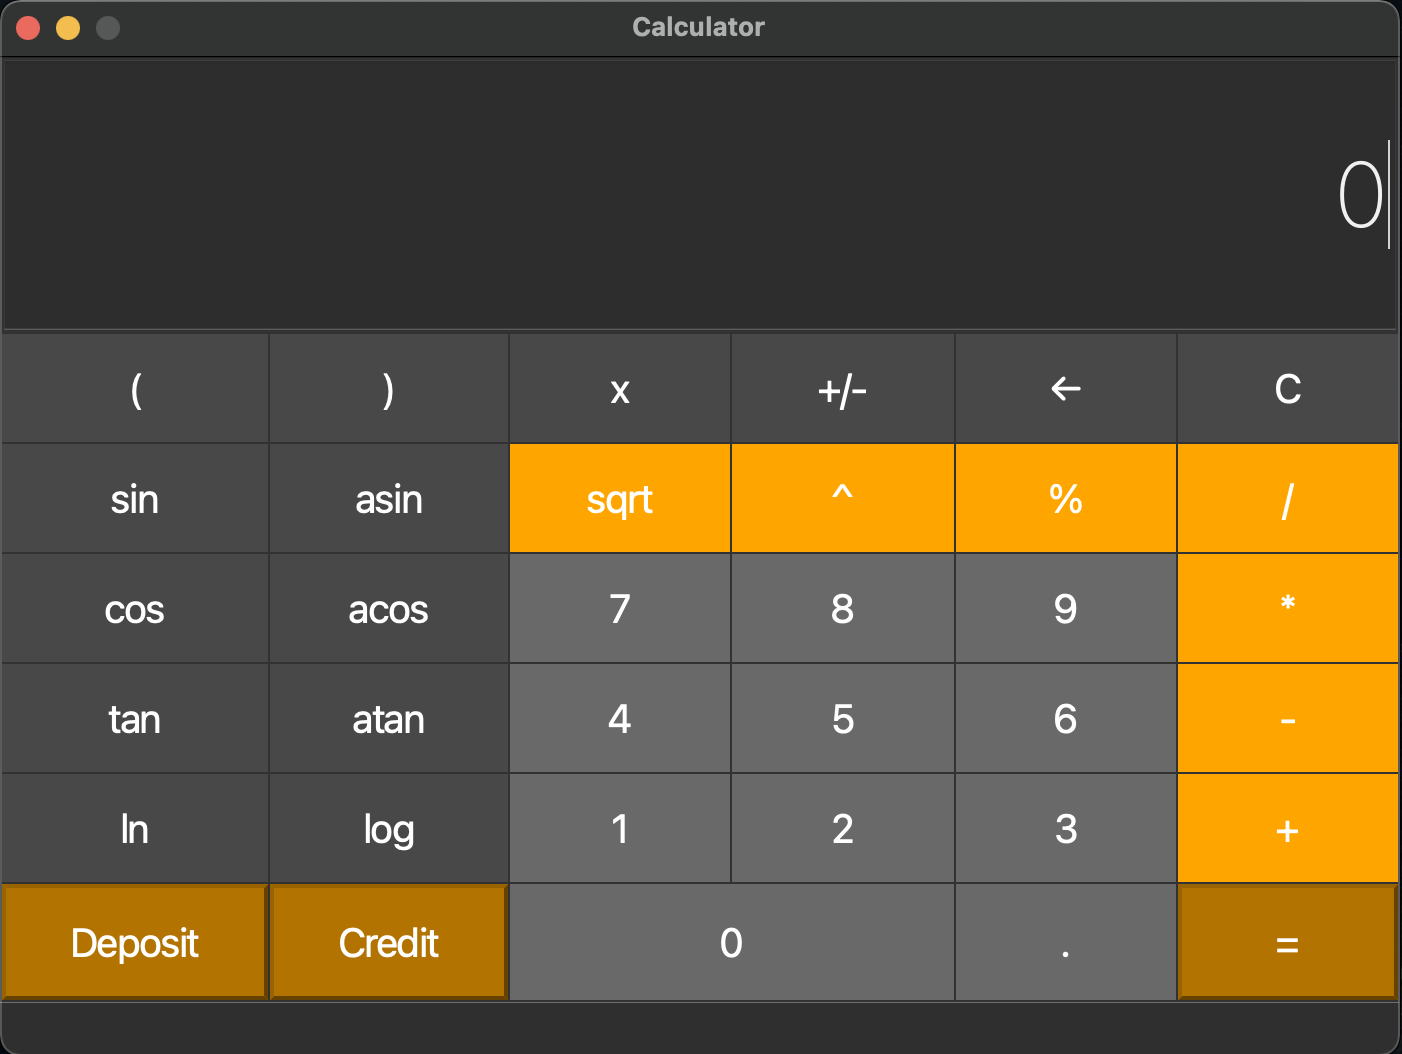
\includegraphics{pics/calc.png}
\caption{Calc}
\end{figure}

\subsection{Deposit calculator}\label{deposit-calculator}

\begin{figure}[htbp]
\centering
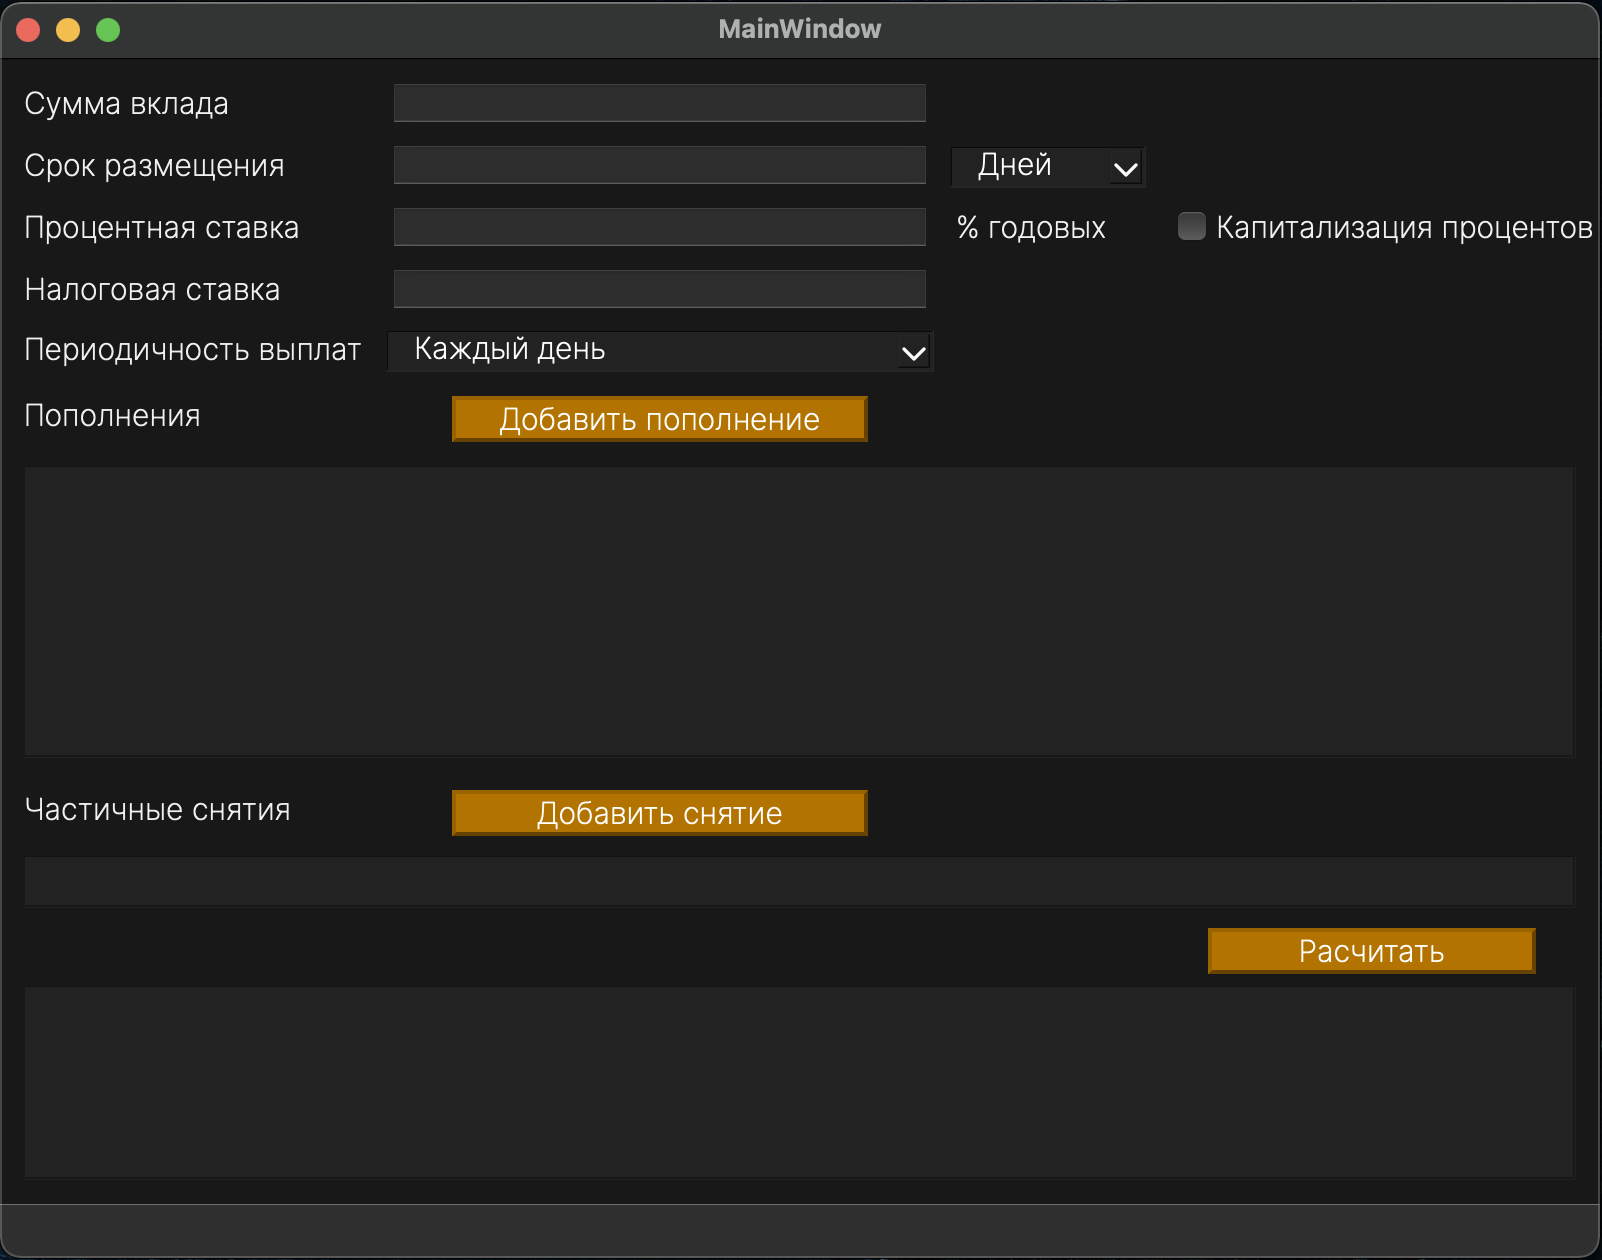
\includegraphics{pics/deposit.png}
\caption{Deposit}
\end{figure}

\subsection{Credit calculator}\label{credit-calculator}

\begin{figure}[htbp]
\centering
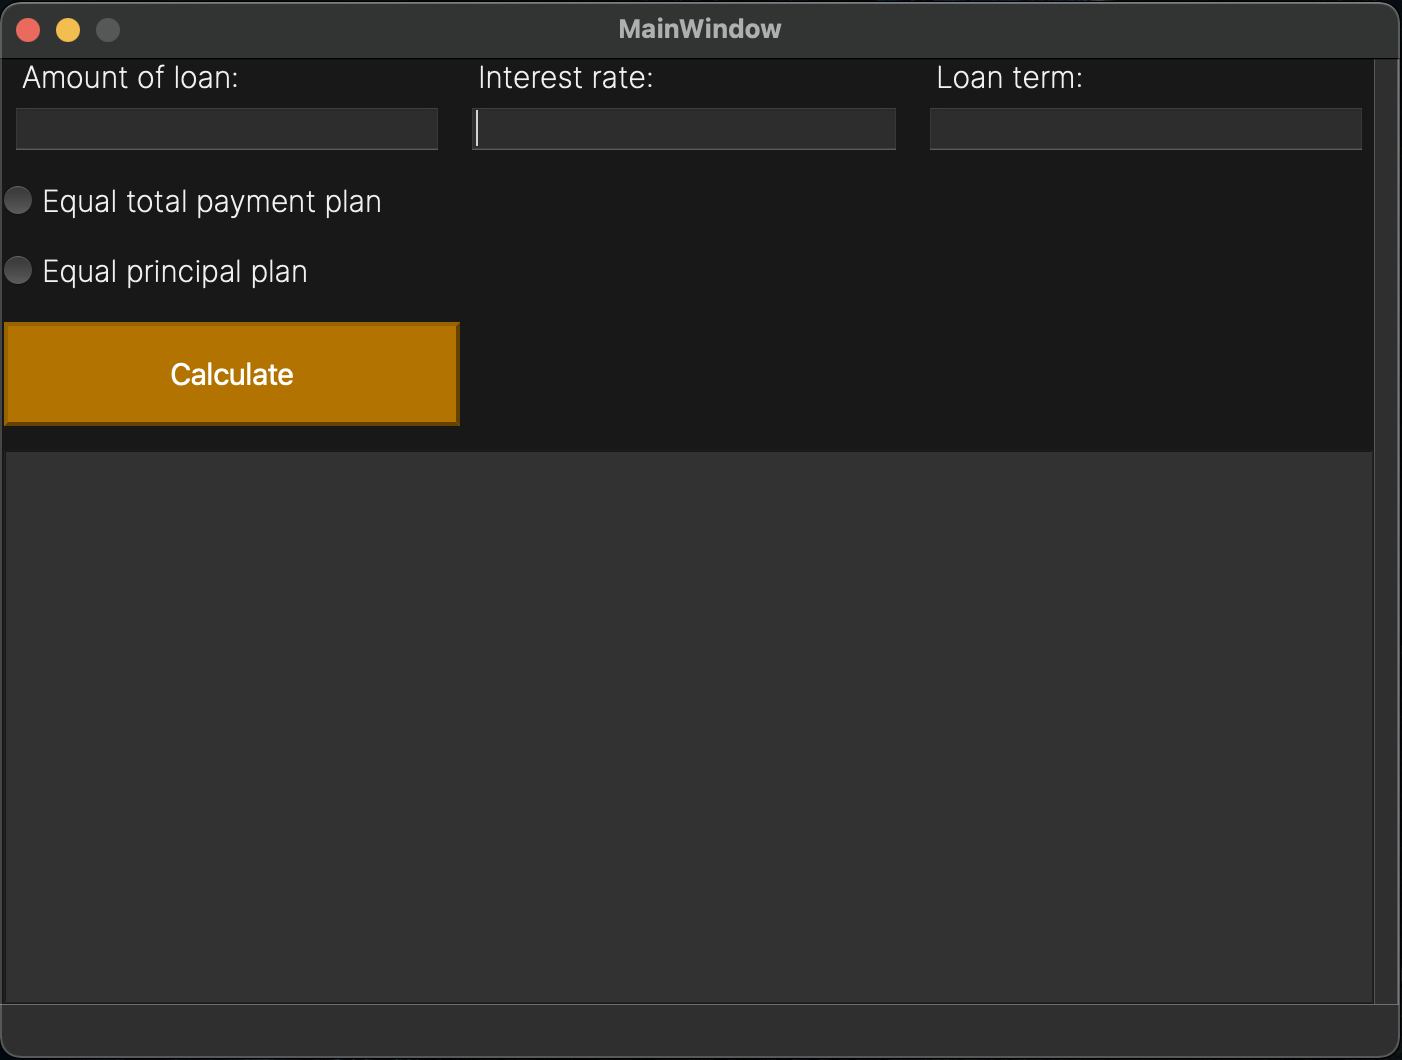
\includegraphics{pics/credit.png}
\caption{Credit}
\end{figure}

\hypertarget{graph}{\subsection{Graph}\label{graph}}

\begin{figure}[htbp]
\centering
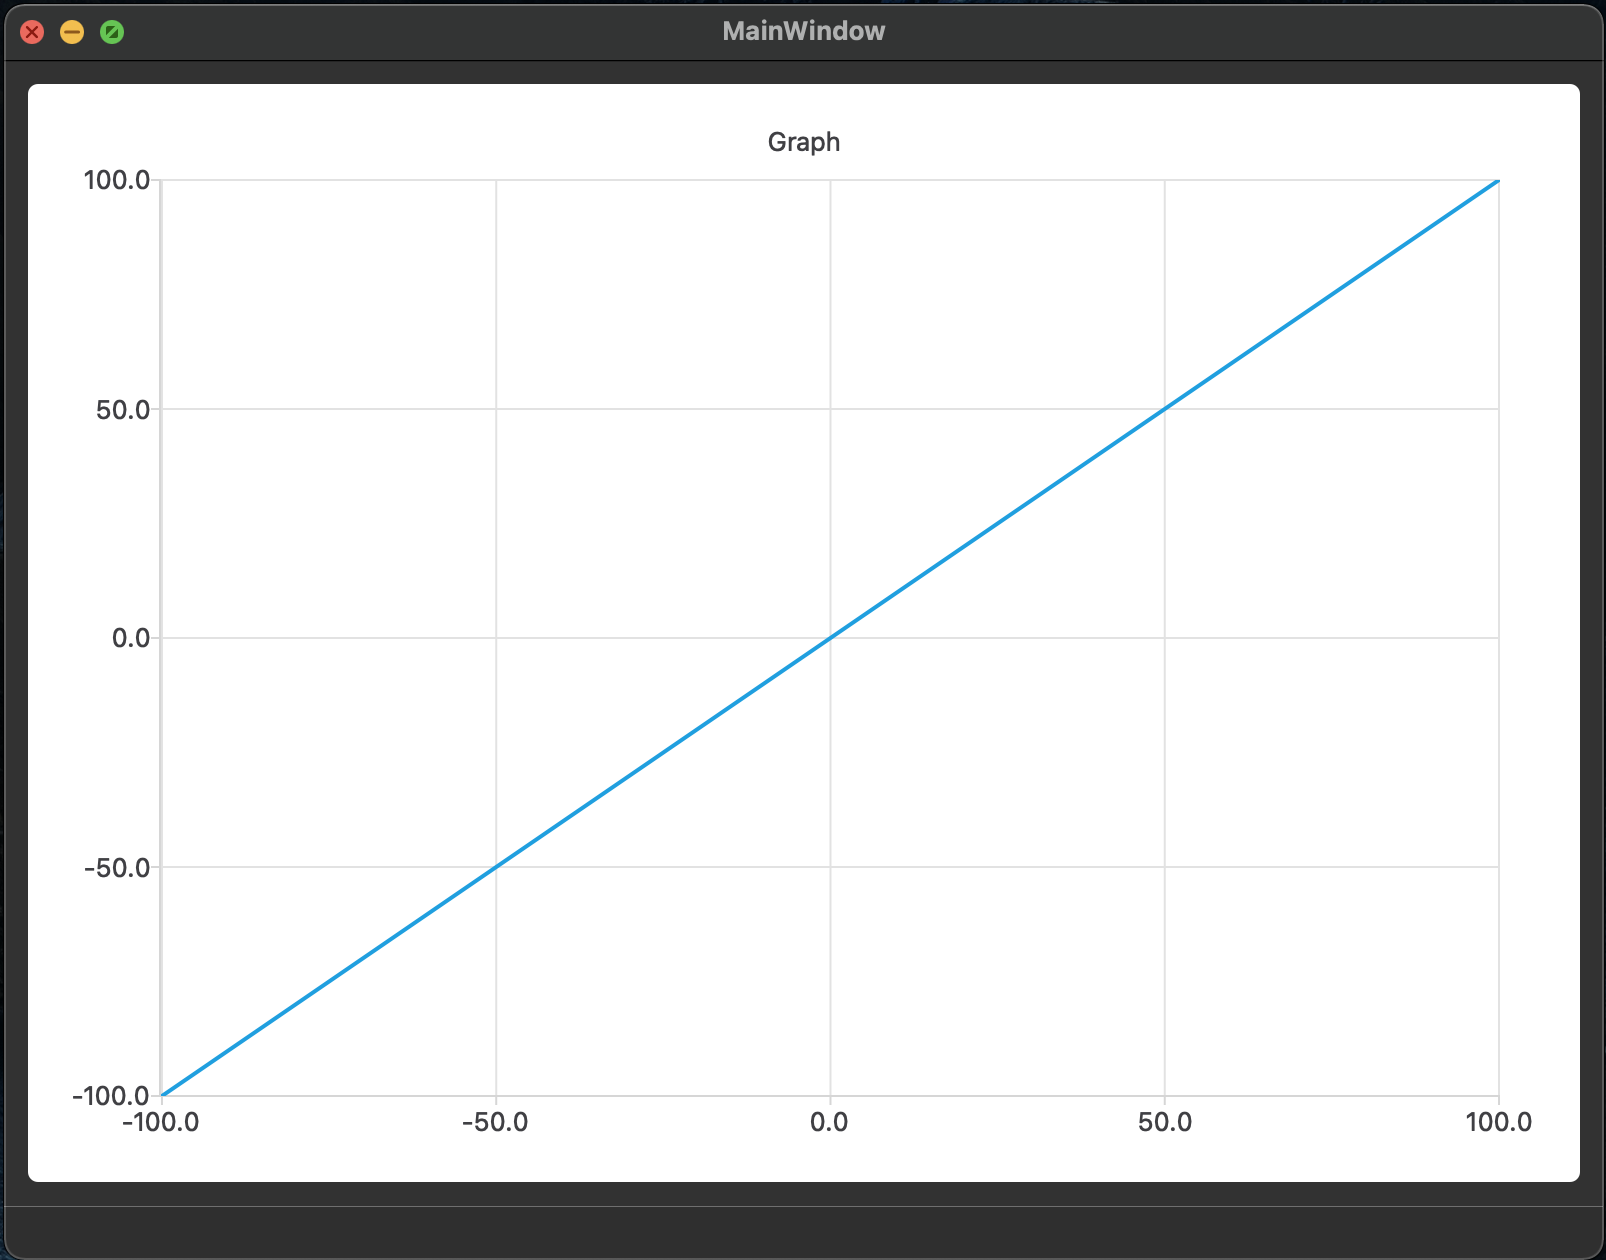
\includegraphics{pics/graph.png}
\caption{Graph}
\end{figure}

\end{document}
